\documentclass[tikz,border=6pt]{standalone}
\usepackage{pgfplots}
\usepgfplotslibrary{groupplots}
\usetikzlibrary{calc}
\pgfplotsset{compat=1.18}
\begin{document}
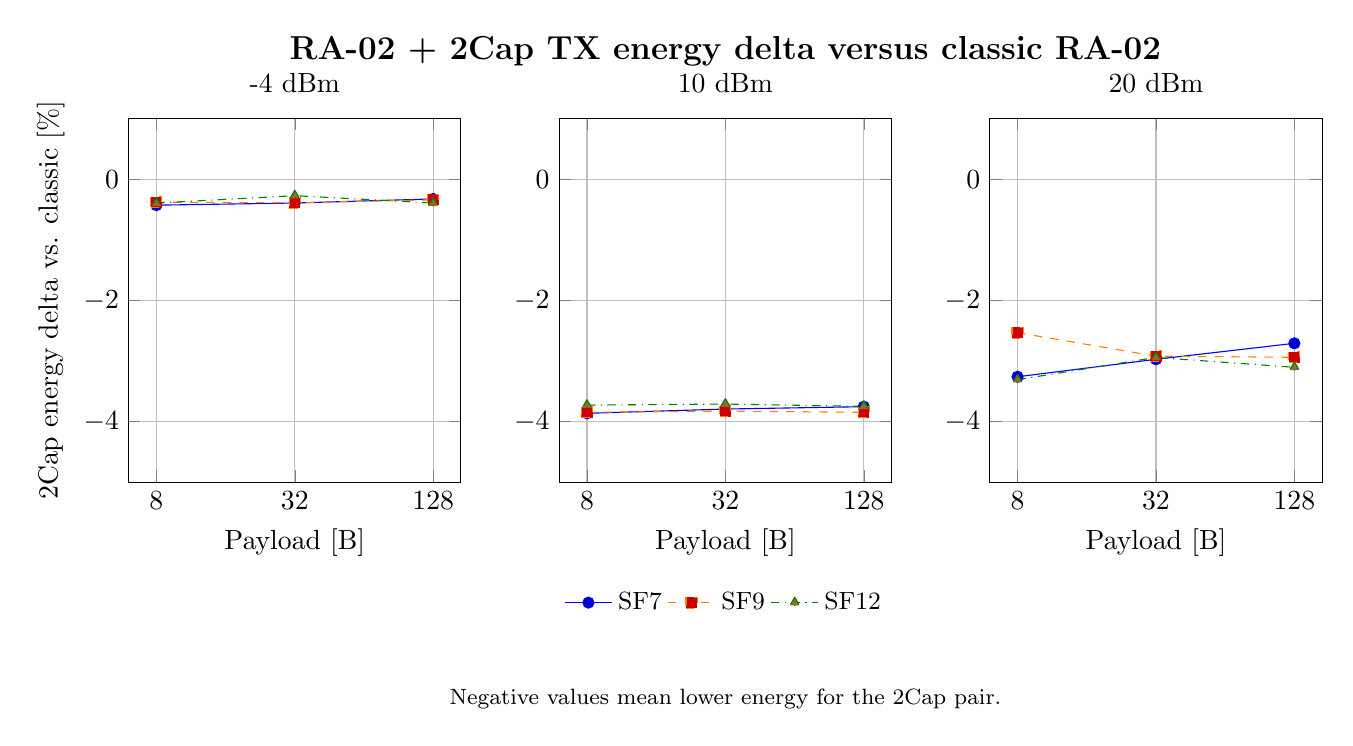
\begin{tikzpicture}
\begin{groupplot}[group style={group size=3 by 1,horizontal sep=1.25cm},
width=5.8cm,height=6.2cm,xmode=log,log basis x=2,ymin=-5,ymax=1,
xtick={8,32,128},xticklabels={8,32,128},grid=both,xlabel={Payload [B]},
legend style={draw=none,fill=none,font=\small,at={(0.5,-0.27)},anchor=north,legend columns=-1}]
\nextgroupplot[title={-4 dBm},ylabel={2Cap energy delta vs. classic [\%]}]
\addplot+[blue,solid,mark=*] coordinates {(8,-0.428545) (32,-0.393127) (128,-0.325722)};
\addplot+[orange,dashed,mark=square*] coordinates {(8,-0.379690) (32,-0.389387) (128,-0.340698)};
\addplot+[green!50!black,dashdotted,mark=triangle*] coordinates {(8,-0.394232) (32,-0.271896) (128,-0.392583)};
\nextgroupplot[title={10 dBm}]
\addplot+[blue,solid,mark=*] coordinates {(8,-3.862961) (32,-3.792309) (128,-3.753460)};
\addlegendentry{SF7}
\addplot+[orange,dashed,mark=square*] coordinates {(8,-3.846705) (32,-3.825928) (128,-3.846268)};
\addlegendentry{SF9}
\addplot+[green!50!black,dashdotted,mark=triangle*] coordinates {(8,-3.727307) (32,-3.710163) (128,-3.747940)};
\addlegendentry{SF12}
\nextgroupplot[title={20 dBm}]
\addplot+[blue,solid,mark=*] coordinates {(8,-3.259888) (32,-2.971744) (128,-2.708013)};
\addplot+[orange,dashed,mark=square*] coordinates {(8,-2.532435) (32,-2.919588) (128,-2.938464)};
\addplot+[green!50!black,dashdotted,mark=triangle*] coordinates {(8,-3.308082) (32,-2.940871) (128,-3.103600)};
\end{groupplot}
\node[font=\bfseries\large] at ($(group c2r1.north)+(0,0.85cm)$) {RA-02 + 2Cap TX energy delta versus classic RA-02};
\node[font=\footnotesize] at ($(group c2r1.south)+(0,-2.75cm)$) {Negative values mean lower energy for the 2Cap pair.};
\end{tikzpicture}
\end{document}
